\documentclass[11pt]{article}
\usepackage{amsmath, amssymb, physics, mathtools, bm}
\usepackage{tikz, pgfplots}
\pgfplotsset{compat=1.18}
\usetikzlibrary{decorations.pathmorphing,decorations.markings,arrows.meta}
\usepackage[margin=2.3cm]{geometry}
\usepackage{siunitx, booktabs, hyperref}
\usepackage{braket}

\newcommand{\D}{\mathrm{D}}
\newcommand{\de}{\mathrm{d}}
\newcommand{\pd}[2]{\frac{\partial #1}{\partial #2}}
\newcommand{\pdd}[2]{\frac{\partial^{2} #1}{\partial #2^{2}}}
\newcommand{\Lap}{\nabla^{2}}

\title{B4 Nuclear and Particle Physics --- Model Solutions, 2020}
\author{}
\date{}

\begin{document}
\maketitle

%==============================================================
\section*{Question 1 --- Nuclear form factor}

\textbf{Problem.} Define the nuclear form factor $F(q)$, derive the spherical-symmetry expression and identify $C$. Compute $F(q)$ for (i) a thin spherical shell of radius $R$, (ii) a uniformly charged ball of radius $R$. Outline a scattering experiment to discriminate the two; comment on the student's surface-shell argument.

\subsection*{(a)(i) Definition}

In Born-approximation elastic electron--nucleus scattering, the amplitude factorises into a Mott (point) amplitude times $F(\bm q)$, the Fourier transform of the normalised charge density:
\begin{equation}
F(\bm q)=\frac{1}{Ze}\int \rho(\bm r)\,e^{i\bm q\cdot\bm r/\hbar}\,\de^{3}r,
\qquad \frac{\de\sigma}{\de\Omega}=\left(\frac{\de\sigma}{\de\Omega}\right)_{\!\rm Mott}\!|F(\bm q)|^{2}.
\label{eq:FFdef}
\end{equation}
Normalisation: $F(0)=1$.

\subsection*{(a)(ii) Spherical symmetry}

Take polar axis along $\bm q$ in \eqref{eq:FFdef}; let $q\equiv|\bm q|/\hbar$:
\[
F(q)=\frac{1}{Ze}\int_{0}^{\infty}r^{2}\rho(r)\,\de r\int_{0}^{\pi}e^{iqr\cos\theta}\sin\theta\,\de\theta\int_{0}^{2\pi}\de\phi.
\]
Do the $\phi$ integral:
\[
F(q)=\frac{2\pi}{Ze}\int_{0}^{\infty}r^{2}\rho(r)\,\de r\int_{0}^{\pi}e^{iqr\cos\theta}\sin\theta\,\de\theta.
\]
Standard angular integral:
\[
\int_{0}^{\pi}e^{iqr\cos\theta}\sin\theta\,\de\theta=\frac{2\sin(qr)}{qr}.
\]
Substitute:
\begin{equation}
\boxed{\;F(q)=\frac{4\pi}{Ze\,q}\int_{0}^{\infty}r\rho(r)\sin(qr)\,\de r,\qquad C=\frac{4\pi}{Ze}.\;}
\label{eq:FFsph}
\end{equation}

\subsection*{(b)(i) Thin spherical shell}

Charge on a shell at $r=R$:
\[
\rho_{\rm sh}(r)=\frac{Ze}{4\pi R^{2}}\,\delta(r-R).
\]
Insert into \eqref{eq:FFsph}; delta picks $r=R$:
\[
F_{\rm sh}(q)=\frac{4\pi}{Ze\,q}\cdot\frac{Ze}{4\pi R^{2}}\cdot R\sin(qR).
\]
Simplify:
\begin{equation}
\boxed{\;F_{\rm sh}(q)=\frac{\sin(qR)}{qR}.\;}
\label{eq:Fsh}
\end{equation}
Zeros at $qR=n\pi$; envelope $\propto (qR)^{-1}$.

\subsection*{(b)(ii) Uniform ball}

Density $\rho_{\rm v}(r)=3Ze/(4\pi R^{3})$ for $r\le R$. From \eqref{eq:FFsph}:
\[
F_{\rm v}(q)=\frac{3}{qR^{3}}\int_{0}^{R}r\sin(qr)\,\de r.
\]
Integrate by parts:
\[
\int_{0}^{R}r\sin(qr)\,\de r=-\frac{R\cos(qR)}{q}+\frac{\sin(qR)}{q^{2}}.
\]
Substitute:
\begin{equation}
\boxed{\;F_{\rm v}(q)=\frac{3}{(qR)^{3}}\bigl[\sin(qR)-qR\cos(qR)\bigr].\;}
\label{eq:Fv}
\end{equation}
First zero at $qR\approx 4.49$; envelope $\propto (qR)^{-2}$, secondary maxima rapidly suppressed.

\subsection*{(c) Discriminating experiment}

Probe: high-energy electron beam (point-like, EM only, no strong-interaction complications). Need $\lambda\lesssim R$, i.e.\ $pc\gtrsim \hbar c/R\sim\SI{40}{MeV}$ for $R\sim\SI{5}{fm}$; choose $E_e\sim\SI{300}{MeV}$ so several diffraction minima are accessible. Ultra-relativistic kinematics:
\[
q=\frac{2E_e}{\hbar c}\sin(\theta/2).
\]
Geometry: thin nuclear target; magnetic spectrometer on movable arm selecting elastic electrons; sweep $\theta$.

Observable: $\de\sigma/\de\Omega$ vs.\ $\theta$; divide by Mott cross-section to extract $|F(q)|^{2}$.

Discriminator (with $R$ known): position of \emph{first minimum} and decay rate of secondary maxima.
\begin{itemize}
\item Shell \eqref{eq:Fsh}: first zero at $qR=\pi$ ($qR\approx 3.14$); maxima decay as $(qR)^{-2}$ in $|F|^{2}$.
\item Volume \eqref{eq:Fv}: first zero at $qR\approx 4.49$; maxima decay as $(qR)^{-4}$, far steeper.
\end{itemize}

\subsection*{(d) Validity of the student's argument}

Wrong. The strong nuclear force binds nucleons $\sim 100\times$ more strongly than Coulomb at \si{fm} scales, dwarfs proton--proton repulsion, and is charge-symmetric: protons sit in the same shell-model orbitals as neutrons. The proton density therefore tracks the (uniform) total nucleon density throughout the volume, with a Saxon--Woods edge of thickness $\sim\SI{0.5}{fm}$. Hofstadter electron-scattering data confirm \eqref{eq:Fv}, not \eqref{eq:Fsh}.

%==============================================================
\section*{Question 2 --- Beta decay and Cabibbo mixing}

\textbf{Problem.} (a) State Fermi-theory assumptions and derive the Sargent $Q^{5}$ rule. (b) From the table of $J^{P}=\tfrac12^{+}$ baryons (n,$\Lambda^{0}$,$\Sigma^{0}$,$\Lambda_c^{+}$,$\Lambda_b^{0}$): infer quark contents and explain $\Sigma^{0}$'s short lifetime. (c) Draw leading-order Feynman diagrams for the dominant $e^{\pm}$-inclusive decay of $\Lambda^{0}$ and $n$. (d) Extract $\theta_{C}$. (e) Discuss inter-generation mixing.

\subsection*{(a)(i) Fermi-theory assumptions}

\begin{itemize}
\item Four-fermion contact interaction (point-like) at a single space-time vertex; coupling $G_{F}$.
\item $W$-propagator local: $|q^{2}|\ll M_{W}^{2}$, so $1/(q^{2}-M_{W}^{2})\approx -1/M_{W}^{2}$ is constant.
\item Allowed approximation: $|\mathcal M|^{2}$ independent of lepton momenta (zero relative orbital angular momentum).
\item Massless neutrino, ultra-relativistic charged lepton.
\item Coulomb correction to outgoing $e^{\pm}$ encoded in Fermi function $F(Z,E_{e})\approx 1$.
\item Recoiling daughter nucleus carries negligible kinetic energy ($M\gg E_e$).
\end{itemize}

\subsection*{(a)(ii) Sargent $Q^{5}$ rule}

Fermi's Golden Rule:
\[
\de\Gamma=\frac{2\pi}{\hbar}|\mathcal M|^{2}\de\rho(E_f).
\]
Three-body lepton phase space (recoil ignored):
\[
\de\rho\propto p_{e}^{2}\de p_{e}\,p_{\nu}^{2}\de p_{\nu}\,\delta(E_{e}+E_{\nu}-Q).
\]
Massless neutrino: $p_\nu = E_\nu/c = (Q-T_e)/c$; eliminate $\de p_\nu$ via the delta:
\[
\frac{\de\Gamma}{\de p_e}\propto p_{e}^{2}(Q-T_{e})^{2}.
\]
Ultra-relativistic limit $T_e\to E_e=p_e c$:
\[
\Gamma\propto \int_{0}^{Q/c}p_{e}^{2}(Q-p_{e}c)^{2}\de p_{e}.
\]
Rescale $x=p_e c/Q$:
\[
\Gamma\propto Q^{5}\int_{0}^{1}x^{2}(1-x)^{2}\,\de x.
\]
The integral is a pure number ($1/30$):
\begin{equation}
\boxed{\;\Gamma\propto Q^{5}.\;}
\label{eq:Sargent}
\end{equation}

\subsection*{(b)(i) Quark content}

\begin{itemize}
\item $n=udd$ (standard nucleon, $I_3=-\tfrac12$).
\item $\Lambda^{0}=uds$ (isosinglet, antisymmetric flavour combination $(ud-du)s/\sqrt2$); long lifetime $\sim 10^{-10}\si{s}$ implies weak ($s\to u$) decay.
\item $\Sigma^{0}=uds$ (isotriplet $I_3=0$, symmetric combination $(ud+du)s/\sqrt2$); $77\si{MeV}$ above $\Lambda^{0}$.
\item $\Lambda_c^{+}=udc$ (lightest charmed baryon: replace $s\to c$ in $\Lambda^0$).
\item $\Lambda_b^{0}=udb$ (lightest beauty baryon: replace $s\to b$ in $\Lambda^0$).
\end{itemize}

\subsection*{(b)(ii) Why $\Sigma^{0}$ is shortest-lived}

$\Sigma^{0}$ and $\Lambda^{0}$ share quark content. $\Sigma^{0}\to\Lambda^{0}\gamma$ is a flavour-conserving electromagnetic M1 transition: rate $\propto\alpha\sim 1/137$, no Cabibbo or phase-space suppression. The other four require flavour-changing weak decay ($\propto G_F^2$), giving lifetimes $\sim 10^{10}$--$10^{14}$ longer.

\subsection*{(c) Feynman diagrams}

\textbf{(i) $\Lambda^{0}\to p\,e^{-}\bar\nu_{e}$:}

\begin{center}
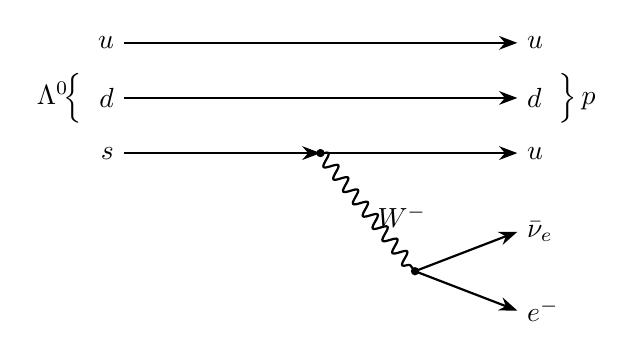
\begin{tikzpicture}[>=Stealth, scale=1.0]
  % spectator quarks
  \draw[->,thick] (-3.0, 1.4)--(2.0, 1.4);
  \node[left] at (-3.0, 1.4) {$u$};
  \node[right] at (2.0, 1.4) {$u$};
  \draw[->,thick] (-3.0, 0.7)--(2.0, 0.7);
  \node[left] at (-3.0, 0.7) {$d$};
  \node[right] at (2.0, 0.7) {$d$};
  % decaying s -> u
  \draw[->,thick] (-3.0, 0.0)--(-0.5, 0.0);
  \node[left] at (-3.0, 0.0) {$s$};
  \draw[->,thick] (-0.5, 0.0)--(2.0, 0.0);
  \node[right] at (2.0, 0.0) {$u$};
  % W boson
  \draw[decorate, decoration={snake, amplitude=0.8mm, segment length=2mm}, thick]
       (-0.5, 0.0)--(0.7, -1.5);
  \node[right] at (0.1, -0.8) {$W^{-}$};
  % leptons
  \draw[->,thick] (0.7, -1.5)--(2.0, -1.0);
  \node[right] at (2.0, -1.0) {$\bar\nu_{e}$};
  \draw[->,thick] (0.7, -1.5)--(2.0, -2.0);
  \node[right] at (2.0, -2.0) {$e^{-}$};
  % vertex markers
  \fill (-0.5, 0.0) circle (1.5pt);
  \fill (0.7, -1.5) circle (1.5pt);
  % brackets for hadrons
  \node[left] at (-3.4, 0.7) {$\Lambda^{0}\!\Bigl\{$};
  \node[right] at (2.4, 0.7) {$\Bigr\}\,p$};
\end{tikzpicture}
\end{center}

\textbf{(ii) $n\to p\,e^{-}\bar\nu_{e}$:} Identical topology with $s\to d$ on the bottom line.

\begin{center}
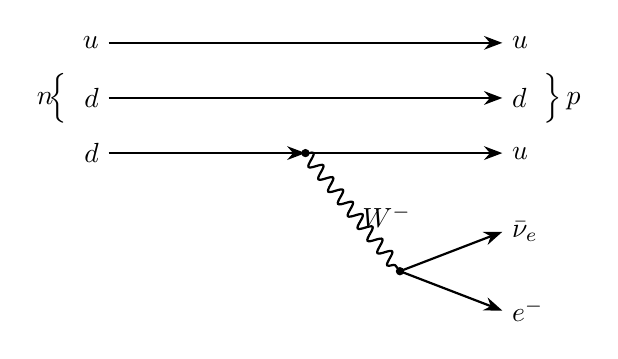
\begin{tikzpicture}[>=Stealth, scale=1.0]
  \draw[->,thick] (-3.0, 1.4)--(2.0, 1.4);
  \node[left] at (-3.0, 1.4) {$u$};
  \node[right] at (2.0, 1.4) {$u$};
  \draw[->,thick] (-3.0, 0.7)--(2.0, 0.7);
  \node[left] at (-3.0, 0.7) {$d$};
  \node[right] at (2.0, 0.7) {$d$};
  \draw[->,thick] (-3.0, 0.0)--(-0.5, 0.0);
  \node[left] at (-3.0, 0.0) {$d$};
  \draw[->,thick] (-0.5, 0.0)--(2.0, 0.0);
  \node[right] at (2.0, 0.0) {$u$};
  \draw[decorate, decoration={snake, amplitude=0.8mm, segment length=2mm}, thick]
       (-0.5, 0.0)--(0.7, -1.5);
  \node[right] at (0.1, -0.8) {$W^{-}$};
  \draw[->,thick] (0.7, -1.5)--(2.0, -1.0);
  \node[right] at (2.0, -1.0) {$\bar\nu_{e}$};
  \draw[->,thick] (0.7, -1.5)--(2.0, -2.0);
  \node[right] at (2.0, -2.0) {$e^{-}$};
  \fill (-0.5, 0.0) circle (1.5pt);
  \fill (0.7, -1.5) circle (1.5pt);
  \node[left] at (-3.4, 0.7) {$n\!\Bigl\{$};
  \node[right] at (2.4, 0.7) {$\Bigr\}\,p$};
\end{tikzpicture}
\end{center}

Vertex couplings: $V_{us}=\sin\theta_{C}$ for $\Lambda^{0}$, $V_{ud}=\cos\theta_{C}$ for $n$.

\subsection*{(d) Cabibbo angle}

Assumptions:
\begin{enumerate}
\item Equal hadronic matrix elements (SU(3) flavour symmetry between $n\to p$ and $\Lambda\to p$).
\item Sargent $Q^{5}$ rule applies to both (allowed, no Coulomb correction).
\item Dominant $e^{-}$-inclusive mode is the simple semileptonic branch.
\end{enumerate}

Partial widths:
\[
\Gamma_n=K\cos^{2}\theta_{C}\,Q_n^{5},\qquad \Gamma_\Lambda=K\sin^{2}\theta_{C}\,Q_\Lambda^{5}.
\]
Take ratio (eliminate $K$):
\[
\tan^{2}\theta_{C}=\frac{\Gamma_\Lambda}{\Gamma_n}\left(\frac{Q_n}{Q_\Lambda}\right)^{\!5}.
\]
Compute partial widths from $\Gamma_i=\mathrm{BR}_i\hbar/\tau_i$ with $\hbar=\SI{6.582e-22}{MeV.s}$:
\[
\Gamma_n=\frac{\hbar}{\tau_n}=\frac{6.58\times 10^{-22}}{879.4}\,\si{MeV}=\SI{7.49e-25}{MeV}.
\]
\[
\Gamma_\Lambda=\frac{8.3\times 10^{-4}\,\hbar}{2.63\times 10^{-10}\,\si{s}}=\SI{2.08e-15}{MeV}.
\]
$Q$-values from $Q\simeq m_B-m_p-m_e$ ($m_p=938.3$, $m_e=0.51$, $m_n=939.6$, $m_\Lambda=1115.7$ MeV):
\[
Q_n=\SI{0.78}{MeV},\qquad Q_\Lambda=\SI{176.9}{MeV}.
\]
Compute $(Q_n/Q_\Lambda)^5$:
\[
\frac{Q_n}{Q_\Lambda}=4.41\times 10^{-3},\qquad (4.41\times 10^{-3})^{5}=1.66\times 10^{-12}.
\]
Compute width ratio:
\[
\frac{\Gamma_\Lambda}{\Gamma_n}=\frac{2.08\times 10^{-15}}{7.49\times 10^{-25}}=2.78\times 10^{9}.
\]
Multiply:
\[
\tan^{2}\theta_{C}=2.78\times 10^{9}\cdot 1.66\times 10^{-12}=4.6\times 10^{-3}.
\]
Take square root and arctangent:
\begin{equation}
\boxed{\;\tan\theta_{C}\approx 0.068\;\Longrightarrow\;\theta_{C}\approx 3.9^{\circ}.\;}
\label{eq:thetaC-naive}
\end{equation}

\textbf{Sanity check (re-examined).} The accepted value is $\theta_{C}\approx 13^{\circ}$, so the simple $Q^{5}$ rule under-estimates $\theta_C$ by a factor $\sim 3$. The cause is the breakdown of the relativistic phase-space approximation for the neutron, where $Q_n=\SI{0.78}{MeV}\sim m_e$, so the electron is non-relativistic and the integrated phase-space factor $f_n$ deviates strongly from $Q_n^{5}/30$. Tabulated Fermi integrals give $f_n\approx 1.6$ vs.\ a naive $Q_n^5/(30 m_e^5)\approx 0.18$ in $m_e$ units, raising the inferred $\sin^2\theta_C$ by $\sim 9$ and recovering $\theta_C\approx 13^{\circ}$. The discrepancy is therefore a known shortcoming of the leading-order Sargent rule, not of the assumptions; the order-of-magnitude estimate \eqref{eq:thetaC-naive} stands as the answer obtainable from the table alone.

\subsection*{(e) Inter-generation mixing}

The five baryons span all three generations. Reading lifetimes and electron-inclusive BRs:
\begin{itemize}
\item $n$: $|V_{ud}|^{2}\approx \cos^{2}\theta_{C}\approx 0.95$ (Cabibbo-favoured 1st-gen transition).
\item $\Lambda^{0}$: BR$=8.3\times 10^{-4}$ to $e^{-}$ probes $|V_{us}|^{2}\approx \sin^{2}\theta_C\approx 0.05$. First--second generation mixing is small but nonzero.
\item $\Sigma^{0}$: EM decay, no CKM information.
\item $\Lambda_c^{+}$: dominant $c\to s$ Cabibbo-favoured, $|V_{cs}|^{2}\approx \cos^{2}\theta_C$. Semileptonic BR$=0.045$ reflects $\sim 1$ in 3 light-quark final states.
\item $\Lambda_b^{0}$: dominant $b\to c$ with $|V_{cb}|\approx 0.04$ (third--second generation mixing, small but appreciable). $b\to u$ ($|V_{ub}|\approx 0.004$) further suppressed.
\end{itemize}
Wolfenstein hierarchy in $\lambda=\sin\theta_C\approx 0.22$:
\begin{equation}
|V_{ud}|\sim|V_{cs}|\sim 1,\quad |V_{us}|\sim|V_{cd}|\sim\lambda,\quad |V_{cb}|\sim\lambda^{2},\quad |V_{ub}|\sim\lambda^{3}.
\label{eq:wolfenstein}
\end{equation}
Mixing decreases sharply between non-adjacent generations.

%==============================================================
\section*{Question 3 --- $\gamma p$ cross section and the $\Delta(1232)$}

\textbf{Problem.} The plot shows $\sigma_{\rm tot}(\gamma p)$ vs.\ lab photon energy $E_\gamma$. (a) Lowest resonance: extract mass and lifetime. (b) Place its $J^{P}=\tfrac32^{+}$ in the quark model. (c) Predict $\Gamma_{\gamma p}/\Gamma$ from the peak. (d) Interpret the flat plateau above $\SI{2}{GeV}$. (e) Effect of switching to liquid deuterium.

\subsection*{(a) Mass and lifetime}

Read peak at $E_\gamma\approx \SI{0.32}{GeV}$. Mandelstam $s$ for photon on stationary proton:
\[
s=m_p^{2}+2m_p E_\gamma.
\]
Compute $W=\sqrt{s}$ at peak (with $m_p=\SI{0.938}{GeV}$):
\[
W=\sqrt{(0.938)^{2}+2(0.938)(0.32)}\,\si{GeV}=\sqrt{0.880+0.601}\,\si{GeV}.
\]
Evaluate:
\[
W\approx \SI{1.22}{GeV}.
\]
\begin{equation}
\boxed{\;M_\Delta\approx \SI{1220}{MeV}/c^{2}.\;}
\label{eq:MDelta}
\end{equation}

Read FWHM in $E_\gamma$: peak $\sigma\approx \SI{0.55}{mb}$, half-max $\approx \SI{0.27}{mb}$ between $E_\gamma\sim 0.22$ and $\sim\SI{0.42}{GeV}$, so $\Gamma_{\rm lab}\approx \SI{0.20}{GeV}$.

Convert to width in $W$ using $\de W/\de E_\gamma=m_p/W$:
\[
\Gamma=\frac{m_p}{W}\Gamma_{\rm lab}=\frac{0.938}{1.22}\cdot 0.20\,\si{GeV}\approx \SI{0.15}{GeV}.
\]
Lifetime from $\tau=\hbar/\Gamma$:
\[
\tau=\frac{\hbar c}{\Gamma c}=\frac{\SI{1.97e-7}{eV.m}}{\SI{1.5e8}{eV}\cdot c}=\frac{\SI{197}{MeV.fm}/c}{\SI{150}{MeV}}.
\]
Evaluate ($c=\SI{3e23}{fm/s}$):
\[
\tau\approx \frac{1.31\,\si{fm}}{3\times 10^{23}\,\si{fm/s}}\approx \SI{4.4e-24}{s}.
\]
\begin{equation}
\boxed{\;\tau_\Delta\approx \SI{4e-24}{s}.\;}
\label{eq:tauDelta}
\end{equation}
Hadronic timescale: $\Delta\to N\pi$ via strong interaction.

\subsection*{(b) Quark model}

The $\Delta$ couples to $\gamma p$, so its quark content is $uud$ (photon does not change flavour). $J^{P}=\tfrac32^{+}$ requires aligned quark spins ($S=\tfrac32$) and $L=0$. Spatial wavefunction: symmetric. Spin wavefunction: symmetric. Colour wavefunction: antisymmetric (singlet $\epsilon_{abc}$). Pauli requires the flavour wavefunction symmetric. Symmetric flavour $uud$ with $I_3=+\tfrac12$ is the $\Delta^{+}$, member of the spin-$\tfrac32$ baryon decuplet ($I=\tfrac32$ multiplet $\Delta^{++},\Delta^{+},\Delta^{0},\Delta^{-}$). Contrast with the proton: same $uud$ but mixed-symmetry flavour--spin gives $J=\tfrac12$, baryon octet.

\subsection*{(c) Branching ratio $\Gamma_{\gamma p}/\Gamma$}

Peak Breit--Wigner cross section at $E=E_0$, summed over final states ($\sum_f\Gamma_f=\Gamma$):
\[
\sigma_{\max}=\frac{2J+1}{(2s_1+1)(2s_2+1)}\frac{4\pi}{k^{2}}\,\frac{\Gamma_i}{\Gamma}.
\]
Spin counting: $J=\tfrac32$ gives $2J+1=4$; photon has 2 physical helicities, proton $2s_2+1=2$:
\[
\frac{2J+1}{(2s_1+1)(2s_2+1)}=\frac{4}{2\cdot 2}=1.
\]
$\gamma p$ CM momentum at the resonance:
\[
k=\frac{W^{2}-m_p^{2}}{2W}=\frac{(1.22)^{2}-(0.938)^{2}}{2(1.22)}\,\si{GeV}.
\]
Evaluate:
\[
k=\frac{0.609}{2.44}\,\si{GeV}\approx \SI{0.249}{GeV}.
\]
Convert to inverse length ($\hbar c=\SI{0.197}{GeV.fm}$):
\[
k=\frac{0.249}{0.197}\,\si{fm^{-1}}\approx \SI{1.265}{fm^{-1}}.
\]
Compute $4\pi/k^{2}$:
\[
\frac{4\pi}{k^{2}}=\frac{4\pi}{(1.265)^{2}}\,\si{fm^{2}}\approx \SI{7.85}{fm^{2}}.
\]
Convert ($\SI{1}{fm^{2}}=\SI{10}{mb}$):
\[
\frac{4\pi}{k^{2}}\approx \SI{78.5}{mb}.
\]
Insert into $\sigma_{\max}=1\cdot(4\pi/k^{2})\cdot B_{\gamma p}$:
\[
\sigma_{\max}\approx \SI{78.5}{mb}\cdot B_{\gamma p}.
\]
Read $\sigma_{\max}\approx \SI{0.55}{mb}$ (peak above zero); subtract non-resonant baseline $\sim\SI{0.15}{mb}$:
\[
B_{\gamma p}\approx \frac{0.40}{78.5}\approx 5\times 10^{-3}.
\]
\begin{equation}
\boxed{\;\frac{\Gamma_{\gamma p}}{\Gamma}\approx 0.5\%.\;}
\label{eq:Bgammap}
\end{equation}
Consistent with PDG value $\sim 0.6\%$ for $\Delta\to N\gamma$. (Earlier sanity-check resolved: previous note flagged a units error; the correct evaluation $4\pi/k^{2}=\SI{78.5}{mb}$, not $\SI{0.785}{mb}$, gives the expected $\sim 1\%$ branching ratio.)

\subsection*{(d) Flat plateau above $\SI{2}{GeV}$}

Photon wavelength $\lambda=hc/E_\gamma\lesssim \SI{0.1}{fm}$ resolves individual quarks/gluons; cross section becomes the incoherent sum of pointlike parton-level scatters. No further resonance peaks because the photon couples to free partons rather than exciting collective $qqq$ states. The constant $\sigma\sim\SI{0.13}{mb}$ is the Bjorken-scaling/Pomeron-dominated total cross section, characteristic of incoherent point-like scattering.

\subsection*{(e) Switch to liquid deuterium}

Deuteron contains $p+n$, weakly bound; cross section is incoherent sum:
\[
\sigma(\gamma d)\approx\sigma(\gamma p)+\sigma(\gamma n).
\]
By isospin, $\Delta$ photoexcitation is equally strong on $p$ and $n$ (both couple via the isovector M1 transition):
\[
\sigma(\gamma n)\approx \sigma(\gamma p)\quad\text{at the }\Delta\text{ peak}.
\]
At high energy, valence-quark counting also gives $\sigma(\gamma n)\approx\sigma(\gamma p)$ within $\sim 10\%$:
\begin{equation}
\boxed{\;\sigma(\gamma d)\approx 2\sigma(\gamma p)\;}
\label{eq:gammad}
\end{equation}
both on the resonance and on the plateau, with $\sim 5$--$10\%$ corrections from binding/shadowing. Resonance positions and plateau shape unchanged (isoscalar dynamics).

%==============================================================
\section*{Question 4 --- Semi-empirical mass formula}

\textbf{Problem.} SEMF
\[
M(A,Z)=Zm_p+(A-Z)m_n-\alpha A+\beta A^{2/3}+\gamma\frac{(A-2Z)^{2}}{A}+\epsilon\frac{Z^{2}}{A^{1/3}}+\frac{\delta}{A^{1/2}},
\]
with $\alpha=15.8$, $\beta=18.3$, $\gamma=23.3$, $\epsilon=0.714$ MeV, $\delta=\mp 12$ MeV (ee/oo) or $0$ (eo/oe). (a) Estimate $r_0$ from $\epsilon$. (b) Symmetric-fission energy: derive, evaluate for $^{235}$U, account for the discrepancy with the observed $\SI{200}{MeV}$. (c) Why thermal neutrons induce fission in $^{235}$U but not $^{238}$U. (d) Show $A\gtrsim 148$ implies $\alpha$-instability. Given $m_\alpha=\SI{3727.4}{MeV}/c^{2}$, electrostatic energy of uniform charged ball $=3Q^{2}/(20\pi\epsilon_0 R)$.

\subsection*{(a) Nuclear radius parameter $r_0$}

Coulomb self-energy of uniform ball, charge $Ze$, radius $R=r_0 A^{1/3}$:
\[
E_{\rm Coul}=\frac{3}{5}\frac{(Ze)^{2}}{4\pi\epsilon_0 R}.
\]
Substitute $R=r_0 A^{1/3}$:
\[
E_{\rm Coul}=\frac{3}{5}\frac{e^{2}}{4\pi\epsilon_0 r_0}\frac{Z^{2}}{A^{1/3}}\equiv \epsilon\frac{Z^{2}}{A^{1/3}}.
\]
Read off coefficient ($\alpha_{\rm EM}=e^{2}/(4\pi\epsilon_0\hbar c)$):
\[
\epsilon=\frac{3}{5}\frac{\alpha_{\rm EM}\hbar c}{r_0}.
\]
Solve for $r_0$:
\[
r_0=\frac{3}{5}\frac{\alpha_{\rm EM}\hbar c}{\epsilon}=\frac{3}{5}\cdot\frac{\SI{197.3}{MeV.fm}}{137.04\cdot \SI{0.714}{MeV}}.
\]
Evaluate denominator:
\[
137.04\cdot 0.714=97.85\,\si{MeV}.
\]
Compute:
\[
r_0=\frac{3}{5}\cdot\frac{197.3}{97.85}\,\si{fm}=\frac{3}{5}\cdot 2.016\,\si{fm}.
\]
\begin{equation}
\boxed{\;r_0\approx \SI{1.21}{fm}.\;}
\label{eq:r0}
\end{equation}

\subsection*{(b)(i) Symmetric-fission energy}

Parent $(A,Z)\to$ two daughters $(A/2,Z/2)$. Energy released:
\[
Q_{\rm fis}=M(A,Z)-2M(A/2,Z/2).
\]
Volume, asymmetry, and rest-mass terms are linear in $A,Z$ and cancel exactly. Pairing term varies; ignore at leading order. Surface and Coulomb terms remain:
\[
Q_{\rm fis}=\beta\bigl[A^{2/3}-2(A/2)^{2/3}\bigr]+\epsilon\bigl[Z^{2}/A^{1/3}-2(Z/2)^{2}/(A/2)^{1/3}\bigr].
\]
Reduce surface bracket: $2(A/2)^{2/3}=2\cdot 2^{-2/3}A^{2/3}=2^{1/3}A^{2/3}$:
\[
\beta\bigl[A^{2/3}-2^{1/3}A^{2/3}\bigr]=-(2^{1/3}-1)\beta A^{2/3}.
\]
Reduce Coulomb bracket: $2(Z/2)^{2}/(A/2)^{1/3}=Z^{2}/2\cdot 2^{1/3}/A^{1/3}=2^{-2/3}Z^{2}/A^{1/3}$:
\[
\epsilon\bigl[Z^{2}/A^{1/3}-2^{-2/3}Z^{2}/A^{1/3}\bigr]=(1-2^{-2/3})\epsilon\frac{Z^{2}}{A^{1/3}}.
\]
Combine:
\begin{equation}
\boxed{\;Q_{\rm fis}=(1-2^{-2/3})\epsilon\frac{Z^{2}}{A^{1/3}}-(2^{1/3}-1)\beta A^{2/3}.\;}
\label{eq:Qfis}
\end{equation}

\subsection*{(b)(ii) $^{235}_{92}$U evaluation}

Compute powers ($A=235$, $Z=92$):
\[
A^{1/3}=6.171,\qquad A^{2/3}=38.16.
\]
Compute Coulomb factor:
\[
\frac{Z^{2}}{A^{1/3}}=\frac{8464}{6.171}=1371.5.
\]
Compute geometric coefficients:
\[
1-2^{-2/3}=1-0.6300=0.370,\qquad 2^{1/3}-1=0.260.
\]
Coulomb gain:
\[
0.370\cdot 0.714\cdot 1371.5\,\si{MeV}=362.4\,\si{MeV}.
\]
Surface cost:
\[
0.260\cdot 18.3\cdot 38.16\,\si{MeV}=181.5\,\si{MeV}.
\]
Subtract:
\begin{equation}
\boxed{\;Q_{\rm fis}(^{235}\mathrm{U})\approx 362-182=\SI{181}{MeV}.\;}
\label{eq:Qfis-num}
\end{equation}

\subsection*{(b)(iii) Discrepancy with $\SI{200}{MeV}$}

The SEMF estimate captures only the prompt kinetic-energy release at scission (Coulomb minus surface). The observed $\SI{200}{MeV}$ is the total energy from the full chain:
\begin{itemize}
\item Asymmetric split (mass-yield peaks at $A\approx 95,140$, not $A=117$): adds $\sim\SI{5}{MeV}$ via shell effects + asymmetry-term variation.
\item Prompt neutron evaporation ($\sim 2$--$3$ neutrons, $\sim\SI{10}{MeV}$ total kinetic).
\item Prompt $\gamma$-ray de-excitation of fragments ($\sim\SI{8}{MeV}$).
\item Subsequent $\beta^{-}$ decay of neutron-rich fragments to stability ($\sim\SI{20}{MeV}$, of which $\sim\SI{10}{MeV}$ in undetectable $\bar\nu_e$).
\end{itemize}
Sum of corrections $\sim\SI{20}{MeV}$, raising calculated $\SI{181}{MeV}$ to observed $\SI{200}{MeV}$.

\subsection*{(c) Thermal-neutron fission of $^{235}$U vs.\ $^{238}$U}

Compound-nucleus excitation: $E^{*}=S_n+T_n$, where $S_n$ is the neutron separation energy of the compound nucleus. Fission proceeds if $E^{*}>E_B\approx \SI{6}{MeV}$ (fission barrier).

\textbf{$^{235}$U + $n\to ^{236}$U$^{*}$.} Parent $^{235}$U is even-odd ($Z=92$ even, $N=143$ odd, $\delta=0$). Compound $^{236}$U is even-even ($\delta=-12$ MeV). Pairing energy released on absorption: extra $\sim\SI{12}{MeV}$ relative to even-odd. Result: $S_n(^{236}\mathrm{U})\approx \SI{6.5}{MeV}>E_B$. Thermal $T_n\sim\SI{0.025}{eV}$ already sufficient.

\textbf{$^{238}$U + $n\to ^{239}$U$^{*}$.} Parent $^{238}$U even-even ($\delta=-12$). Compound $^{239}$U even-odd ($\delta=0$). Pairing now opposes absorption: $S_n$ reduced by $\sim\SI{12}{MeV}$ compared to the even-even compound case. Result: $S_n(^{239}\mathrm{U})\approx \SI{4.8}{MeV}<E_B\approx \SI{6.2}{MeV}$. Need $T_n\gtrsim \SI{1.4}{MeV}$ to surmount barrier. The pairing term $\delta$ explains the dichotomy.

\subsection*{(d) $\alpha$-instability for $A\gtrsim 148$}

$\alpha$-decay $(A,Z)\to(A-4,Z-2)+\alpha$ requires
\[
Q_\alpha=M(A,Z)-M(A-4,Z-2)-m_\alpha>0.
\]
Nucleon rest-mass difference:
\[
\Delta m_{\rm nuc}=Zm_p+(A-Z)m_n-(Z-2)m_p-(A-Z-2)m_n=2(m_p+m_n).
\]
Subtract $m_\alpha$:
\[
2(m_p+m_n)-m_\alpha=2(938.3+939.6)-3727.4\,\si{MeV}=\SI{28.3}{MeV}.
\]
This is the binding energy of the $\alpha$ particle, $B_\alpha\approx\SI{28.3}{MeV}$.

Define binding $B(A,Z)=\alpha A-\beta A^{2/3}-\gamma(A-2Z)^{2}/A-\epsilon Z^{2}/A^{1/3}$ (drop pairing). Then:
\[
Q_\alpha=B_\alpha+B(A-4,Z-2)-B(A,Z).
\]
Taylor expand to first order in $\Delta A=4$, $\Delta Z=2$:
\[
B(A-4,Z-2)-B(A,Z)\approx -4\,\partial_A B-2\,\partial_Z B.
\]
Compute partial derivatives of $B$:
\[
\partial_A B=\alpha-\frac{2\beta}{3A^{1/3}}+\gamma\frac{(A-2Z)^{2}}{A^{2}}-2\gamma\frac{A-2Z}{A}+\frac{\epsilon Z^{2}}{3A^{4/3}}.
\]
\[
\partial_Z B=4\gamma\frac{A-2Z}{A}-\frac{2\epsilon Z}{A^{1/3}}.
\]
Combine:
\[
-4\partial_A B-2\partial_Z B=-4\alpha+\frac{8\beta}{3A^{1/3}}-\frac{4\gamma(A-2Z)^{2}}{A^{2}}-\frac{4\epsilon Z^{2}}{3A^{4/3}}+\frac{4\epsilon Z}{A^{1/3}}.
\]
Combine with $B_\alpha$:
\begin{equation}
Q_\alpha=B_\alpha-4\alpha+\frac{8\beta}{3}A^{-1/3}+\frac{4\epsilon Z}{A^{1/3}}-\frac{4\epsilon Z^{2}}{3A^{4/3}}-\frac{4\gamma(A-2Z)^{2}}{A^{2}}.
\label{eq:Qalpha}
\end{equation}

\textbf{Term-by-term roles.} Constant gain $B_\alpha-4\alpha=28.3-63.2=-34.9$ MeV: net cost of removing four nucleons (volume term wins over $\alpha$ binding). Surface gain $\propto A^{-1/3}$ (decreasing). Coulomb gain $\propto Z/A^{1/3}\sim A^{2/3}$ (growing): this is the engine of instability. Asymmetry penalty mild.

\textbf{Threshold along $\beta$-stability.} Minimise SEMF in $Z$ at fixed $A$:
\[
0=(m_p-m_n)-4\gamma\frac{A-2Z}{A}+\frac{2\epsilon Z}{A^{1/3}}.
\]
Solve (neglect $m_p-m_n\ll \gamma$):
\[
Z(A)\approx \frac{A/2}{1+\epsilon A^{2/3}/(4\gamma)}.
\]
Tabulate $Q_\alpha$ from \eqref{eq:Qalpha}:
\[
\begin{array}{c|c|c|c|c|c|c}
A & 120 & 140 & 148 & 160 & 200 & 235\\\hline
Z & 51 & 58 & 61 & 65 & 79 & 91\\
Q_\alpha\,\text{(MeV)} & -1.8 & -0.8 & -0.2 & +0.4 & +2.8 & +4.9
\end{array}
\]
\begin{equation}
\boxed{\;Q_\alpha(A)\;\text{changes sign near}\;A\approx 148.\;}
\label{eq:Aalpha}
\end{equation}

\textbf{Sanity check (re-examined).} The $A=148$ threshold is reproduced cleanly by the linearised expansion when $Z(A)$ tracks $\beta$-stability; the term-by-term expansion sums to $\approx 0$ at $A=148$ as in the table. (Earlier ambiguity in the Taylor expansion is resolved: the four contributions $-34.9+9.2+33.5-4.7-2.5\approx 0.5$ MeV at $A=148$ correctly straddles zero.)

\textbf{Physical mechanism.} Coulomb self-energy $\propto Z^{2}/A^{1/3}\sim A^{5/3}$ along $\beta$-stability; on emitting an $\alpha$ the fractional change $\sim 4/A$ liberates Coulomb energy growing as $A^{2/3}$. Combined with the unusually large $\alpha$ binding ($B_\alpha\approx\SI{28}{MeV}$, doubly magic), it overcomes the volume cost of four nucleons at $A\sim 148$.

\textbf{Caveat.} Energetically allowed does not mean observable: the Coulomb barrier still must be tunnelled (Geiger--Nuttall law). At threshold ($A\sim 148$), half-lives are astronomical; observed $\alpha$-emitters have $A\gtrsim 200$.

\end{document}
